\section{Methods}
\label{sec:method}

\subsection{Participants}
Ten right-handed healthy subjects participated in this experiment (three females, seven males; age: 19$-$26 years (mean = 20.9 years; S.E. = 2.1 years)). The experiment was approved by the ethical committee of the Faculty of Social Sciences of the Radboud University and all the participants gave informed consent.\\
\\
Participants were primarily found amongst AI students at the Radboud University. Participants were excluded from the experiment when they exhibit certain symptoms or disorders, amongst epilepsy and dyslexia. The following exclusion criteria were used:
\begin{itemize}
	\item Cognitive deficits that made comprehension of the information letter and intructions difficult, or motor impairment that made comprehension of the task or pushing a button impossible.
	\item Epilepsy. We used flickering stimuli in the experiment.
	\item Dyslexia. We used artificial words in the experiment and the participant should have no trouble distinguishing between letters and registering the order of letters.
\end{itemize}

\subsection{Experimental paradigm}
%procedure


%paradigm


%\begin{figure}[h]
%	\centering
%	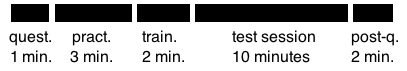
\includegraphics[width=\textwidth]{media/timeline-experiment}
%	\caption{Figure \ref{fig:timeline} shows the estimated timeline, not including breaks, of the experiment. The experiment starts with the BIT, capfitting, calibrating the eyetracker and a practice session. The second session 'before prism' starts immediately after. The third session 'after prism' starts with 15 minutes of prism adaptation and the first 20 trials, followed by two times 10 minutes of prism adaptation and 20 trials.}
%	\label{fig:timeline}
%\end{figure}

%task
\subsubsection{Task}
\label{sec:task}


%\begin{figure}[h]
%	\centering
%	\includegraphics[width=\textwidth]{media/screenshots}
%	\caption{The timeline of a single trial is shown. The baseline is the fixation cross. The cue for direction of attention is given and the stimuli commence. After the stimuli, the system asks the participant how many Xs he has counted at the attended side and feedback is shown immediately after.}
%	\label{fig:screenshots}
%\end{figure}

%feedback
\subsubsection{Feedback}
\label{sec:feedback}




\subsection{Eyetracker}


\subsection{Preprocessing}


\subsection{Statistical analysis}

